\documentclass{VUMIFInfBakalaurinis}
\usepackage{algorithmicx}
\usepackage{algorithm}
\usepackage{algpseudocode}
\usepackage{amsfonts}
\usepackage{amsmath}
\usepackage{bm}
\usepackage{caption}
\usepackage{color}
\usepackage{float}
\usepackage{graphicx}
% \usepackage{hyperref}  % Nuorodų aktyvavimas
\usepackage{listings}
\usepackage{subfig}
\usepackage{url}
\usepackage{wrapfig}

\usepackage{longtable}

% Titulinio aprašas
\university{Vilniaus universitetas}
\faculty{Matematikos ir informatikos fakultetas}
\department{Programų sistemų katedra}
\papertype{Baigiamasis bakalauro darbas}
\title{Dalykinės srities modelio transformavimas į UML sekų diagramas}
\titleineng{Deriving use cases from business process}
\status{4 kurso 1 grupės studentas}
\author{Aleksandras Sivkovas}
% \secondauthor{Vardonis Pavardonis}   % Pridėti antrą autorių
\supervisor{Prof. dr. Saulius Gudas}
\reviewer{prof. habil. dr. Vardaitis Pavardaitis}
\date{Vilnius \\ \the\year}

% Nustatymai
% \setmainfont{Palemonas}   % Pakeisti teksto šriftą į Palemonas (turi būti įdiegtas sistemoje)
\bibliography{bibliografija} 

\begin{document}
\maketitle

\tableofcontents

%Sutartinių ženklų, simbolių, vienetų ir terminų sutrumpinimų sąrašas (jeigu
%ženklų, simbolių, vienetų ir terminų bendras skaičius didesnis nei 10 ir
%kiekvienas iš jų tekste kartojasi daugiau nei 3 kartus).
\sectionnonum{Sąvokų apibrėžimai}
Šiame darbe naudojami žymėjimai:
\begin{enumerate}
	\item \textbf{BPMN} – modeliavimo kalba, skirta pavaizduoti informaciją plačiai auditorijai. \textbf{BPMN} buvo sukurta ir dažniausia naudojama pavaizduoti verslo procesams \cite{bpmnFormal}.
	\item \textbf{UML} – modeliavimo kalba, skirta suteikti standartinį sistemos analizės, architektūros, veikimo ir kūrimo pavaizdavimą \cite{omgUmlFormal}.
	\item \textbf{Sekų diagrama} – \textbf{UML} diagrama, skirta pavaizduoti žinučių tarp apibrėžtų objektų sekai tų objektų gyvavimo metu \cite{omgUmlFormal}.
\end{enumerate}


%Įvade apibūdinamas darbo tikslas, temos aktualumas ir siekiami rezultatai.
\sectionnonum{Įvadas}
Darbo tikslas – apibrėžti ir įgyvendinti algoritmą \textbf{BPMN} modelio transformacijai į \textbf{sekų diagramas}.

Reikalavimų inžinerija yra sudėtinga programų kūrimo dalis. Proceso sudėtingumas dažnai tampa klaidų priežastimi. Čia atsiradusios klaidos sunkiai aptinkamos ir sukelia brangiai kainuojančias pasekmes, nes sekančiuose etapuose bus kuriama neteisingai apibrėžta programa. Norint išvengti klaidų galima kai kurias proceso veiklas automatizuoti.

Darbe bus tiriama verslo proceso transformacija į kuriamos programos \textbf{sekų diagramas}. \textbf{Sekų diagramos} yra svarbi reikalavimų inžinerijos dalis, kadangi ji apibrėžia kokios transakcijos vyks programų sistemoje. Įmonės dažniausiai žino kaip ir kokias veiklas jos vykdo. Verslo procesą galima apibrėžti \textbf{BPMN} diagramomis. Bet ne viską, kas yra \textbf{BPMN} modelyje, galima perkelti į \textbf{sekų diagramą}, todėl darbe bus apibrėžtas suprastintas \textbf{BPMN} modelis, kuriame bus vaizduojama tik algoritmui aktuali informacija. Čia bus tiriama \textbf{BPMN} modelio transformacijos į \textbf{sekų diagramas} algoritmas.

Siekiami rezultatai yra:
\begin{enumerate}
	\item Suprastinto \textbf{BPMN} modelio apibrėžimas.
	\item Algoritmas galintis transformuoti \textbf{BPMN} modelį į \textbf{sekų diagramą}.
	\item Programa demonstruojanti algoritmo veikimą.
\end{enumerate}


%Pagrindinėje tiriamojoje dalyje aptariama ir pagrindžiama tyrimo metodika;
%pagal atitinkamas darbo dalis, nuosekliai, panaudojant lyginamosios analizės,
%klasifikacijos, sisteminimo metodus bei apibendrinimus, dėstoma sukaupta ir
%išanalizuota medžiaga. 
\section{Tiriamų modelių apibrėžimai}
Kadangi darbe bus tiriama vienos diagramos transformacija į kitą, pirmiausia pateikiami jų apibrėžimai.

%Citavimo pavyzdžiai: cituojamas vienas šaltinis \cite{PvzStraipsnLt}; cituojami
%keli šaltiniai \cite{PvzStraipsnEn, PvzKonfLt, PvzKonfEn, PvzKnygLt, PvzKnygEn,
%PvzElPubLt, PvzElPubEn, PvzMagistrLt, PvzPhdEn}.
\subsection{BPMN diagrama}
\textbf{BPMN} specifikacija leidžia atvaizduoti gana nemažai verslo proceso atributų \cite{bpmnFormal}. Bet šiame darbe ji bus nagrinėjama tik kaip įvesties duomenų formatas, naudojamas apibrėžti informaciją pagal kurią bus kuriama \textbf{sekų diagrama}. Taigi daugelį \textbf{BPMN} komponentų galima tiesiog ignoruoti, nes jie neturi jokios įtakos algoritmo vykdymo rezultatui. Norint pabrėžti svarbią informaciją, darbe bus tiriamos tik tos \textbf{BPMN} savybės kurios gali įtakoti algoritmo vykdymo rezultatą. Atitinkami komponentai pavaizduoti \ref{tab:investigated_bpmn_components} lentelėje.
\newcounter{counter:table:reset}
\newcounter{counter:table}[counter:table:reset]
\newcommand\rownumber{\stepcounter{counter:table}\arabic{counter:table}}
\begin{center}
    \begin{longtable}{ | p{0.5cm} | p{2cm} |  p{7cm} | p{4cm} |}
    \caption{BPMN diagramos komponentai}
	\label{tab:investigated_bpmn_components}
    \\ \hline 
    Nr. & Komponentas & Aprašymas & Žymėjimo pavizdys\\ 
    \hline 
    \rownumber & Rolė & Komponentas žymintis diagramos dalyvį ir nurodantis, kad jis atsakingas už veiklų esančių šiame komponente vykdymą. & \vtop{\hbox{\strut }\hbox{\strut 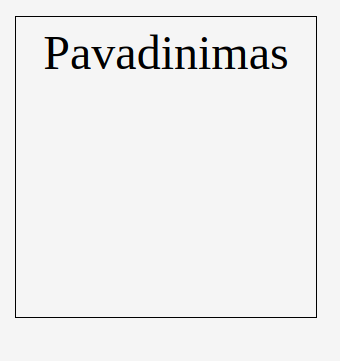
\includegraphics[width=3cm]{img/bpm-components/pool}}} \\
    \hline
     \rownumber & Įvykis & Komponentas žymintis, kad ivyko kažkas kas įtakojo proceso būseną. & \vtop{\hbox{\strut }\hbox{\strut 
\includegraphics[width=3cm]{img/bpm-components/event}}} \\ 
    \hline 
    \rownumber & Veikla & Komponentas žymintis užduoties vykdymo procesą & \vtop{\hbox{\strut }\hbox{\strut 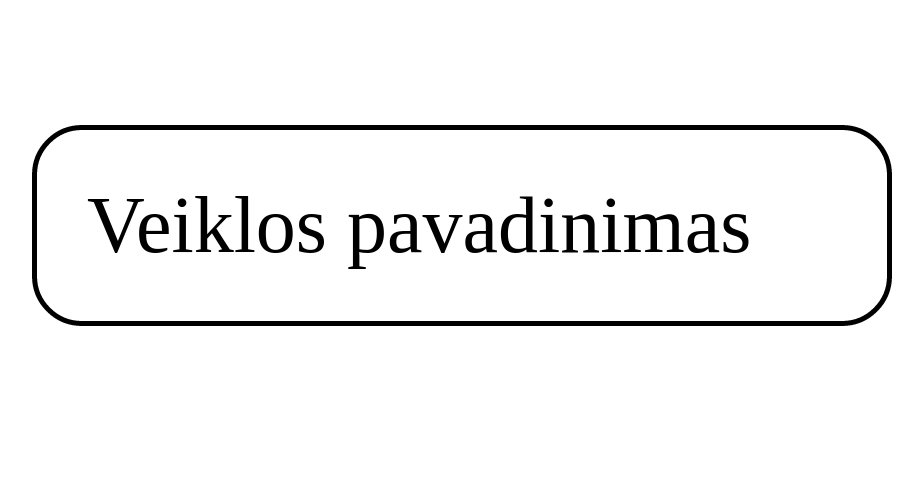
\includegraphics[width=3cm]{img/bpm-components/activity}}}\\
    \hline 
    \rownumber & Sekos srautas & Komponentas žymintis veiklų seką. & \vtop{\hbox{\strut }\hbox{\strut 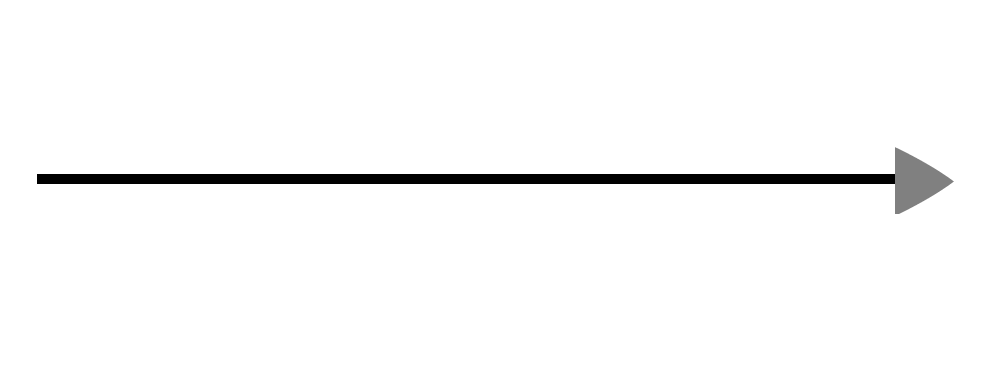
\includegraphics[width=3cm]{img/bpm-components/transition}}}\\
    \hline
    \rownumber & Duomenų objektas & Komponentas žymintis sukuriamus arba įeities duomenis. & \vtop{\hbox{\strut }\hbox{\strut 
\includegraphics[width=3cm]{img/bpm-components/data_object}}}\\
    \hline
    \rownumber & Pranešimų srautas & Komponentas žymintis duomenų apsikeitimo srautus. & \vtop{\hbox{\strut }\hbox{\strut 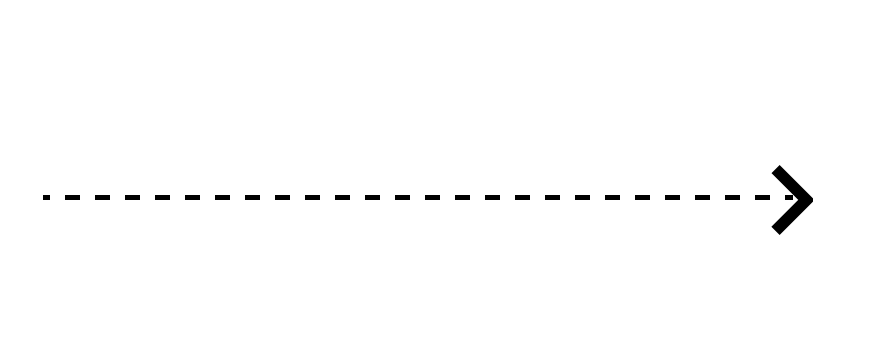
\includegraphics[width=3cm]{img/bpm-components/message_flow}}}\\
    \hline
    \rownumber & Sprendimas & Komponentas žymintis sekos srautų išsišakojimą. & \vtop{\hbox{\strut }\hbox{\strut 
\includegraphics[width=3cm]{img/bpm-components/gateway}}}\\
    \hline
    \end{longtable}
\end{center}


\subsection{Sekų diagrama}

Kaip ir \textbf{BPMN} atveju \textbf{sekų diagrama} turi komponentus, kurie nebus nagrinėjami šiame darbe. \ref{tab:investigated_sequence_diagram_components} lentelė vaizduoja kas bus tiriama iš sekų diagramos.
\stepcounter{counter:table:reset}
\begin{center}
    \begin{longtable}{ | p{0.5cm} | p{2cm} |  p{7cm} | c |}
    \caption{Sekų diagramos komponentai}
	\label{tab:investigated_sequence_diagram_components}
    \\ \hline 
    Nr. & Komponentas & Aprašymas & Žymėjimo pavizdys\\ 
    \hline 
    \rownumber & Gyvavimo linija & Komponentas žymintis diagramos objekto dalyvavimo laiką procese. & \vtop{\hbox{\strut }\hbox{\strut 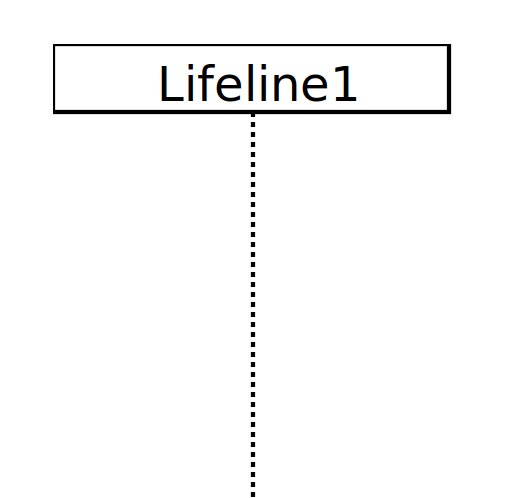
\includegraphics[width=3cm]{img/sequence-diagram-components/lifeline}}} \\
    \hline
    \rownumber & Vykdymo specifikacija & Komponentas žymintis sinchroninio pranešimo tranzakciją. & \vtop{\hbox{\strut }\hbox{\strut 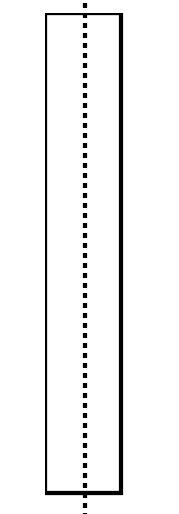
\includegraphics[height=3cm]{img/sequence-diagram-components/execution_specification}}} \\
    \hline
     \rownumber & Žinutė & Komponentas žymintis duomenų perdavimą iš vieno dalyvio į kitą & \vtop{\hbox{\strut }\hbox{\strut 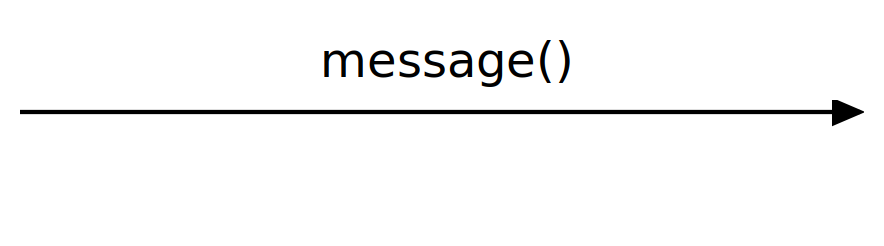
\includegraphics[width=3cm]{img/sequence-diagram-components/message}}} \\
    \hline
     \rownumber & Atsakymas & Komponentas žymintis, kad dalyvis sureagavo į sinchroninę užduotį. & \vtop{\hbox{\strut }\hbox{\strut 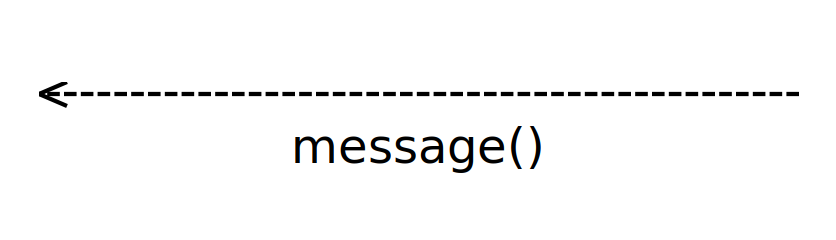
\includegraphics[width=3cm]{img/sequence-diagram-components/reply-message}}} \\
    \hline
    \end{longtable}
\end{center}

\section{Algoritmas kurti sekų diagramas pagal BPMN pateiktą informaciją}
Šio darbo tikslas yra algoritmas atlikti diagramų transformacijai. Pirmiausia pateikiama tai kas literatūroje rašoma apie UML diagramų transformavimo algoritmus. Vėliau sukuriamas siekiamas algoritmas.
\subsection{UML diagramų transformavimo algoritmai}
\subsubsection{Vartojimo atvejų diagramos išvedimas iš BPMN modelio}
Literatųroje yra parašyta apie vartojimo atvejų diagramos išvedimą iš BPMN modelio \cite{algUseCasesFromBpmn}.
\subsection{Sekų diagramos išvedimas iš BPMN modelio}
\section{Programa BPMN transformacijai į sekų diagramą}   


%Išvadose ir pasiūlymuose, nekartojant atskirų dalių apibendrinimų,
%suformuluojamos svarbiausios darbo išvados, rekomendacijos bei pasiūlymai.
\sectionnonum{Išvados}

%Šiame skyriuje pateikiamos išvados (reziume) anglų kalba.
\sectionnonum{Conclusions}


% bibliografija.bib faile. Šaltinių sąraše nurodoma panaudota literatūra,
% kitokie šaltiniai. Abėcėlės tvarka išdėstoma tik darbe panaudotų (cituotų,
% perfrazuotų ar bent paminėtų) mokslo leidinių, kitokių publikacijų
% bibliografiniai aprašai (šiuo punktu pasirūpina LaTeX). Aprašai pateikiami
% netransliteruoti.
\printbibliography[heading=bibintoc] % Literatūros šaltiniai aprašomi


% Prieduose gali būti pateikiama pagalbinė, ypač darbo autoriaus savarankiškai
% parengta, medžiaga. Savarankiški priedai gali būti pateikiami kompiuterio
% diskelyje ar kompaktiniame diske. Priedai taip pat vadinami ir numeruojami.
% Tekstas su priedais siejamas nuorodomis (pvz.: \ref{img:mlp}).
\appendix  % Priedai


%\section{Niauroninio tinklo struktūra}
%\begin{figure}[H]
%    \centering
%    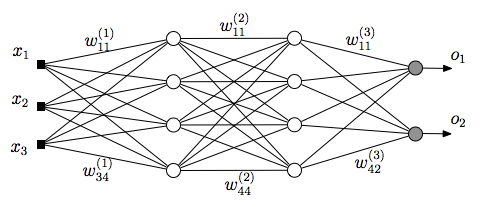
\includegraphics[scale=0.5]{img/MLP}
%    \caption{Paveikslėlio pavyzdys}
%    \label{img:mlp}
%\end{figure}


%\section{Eksperimentinio palyginimo rezultatai}
% tablesgenerator.com - converts calculators (e.g. excel) tables to LaTeX
%\begin{table}[H]\footnotesize
%  \centering
%  \caption{Lentelės pavyzdys}
%  {\begin{tabular}{|l|c|c|} \hline
%    Algoritmas & $\bar{x}$ & $\sigma^{2}$ \\
%    \hline
%    Algoritmas A  & 1.6335    & 0.5584       \\
%    Algoritmas B  & 1.7395    & 0.5647       \\
%    \hline
%  \end{tabular}}
%  \label{tab:table example}
%\end{table}

\end{document}
